\setcounter{figure}{0}
\setcounter{table}{0}
\renewcommand{\thefigure}{S\arabic{figure}}
\renewcommand{\thetable}{S\Roman{table}}

\section*{Supplemental Material}

\subsection*{Simulations of A/H3N2-like populations}

\begin{figure*}[h]
  \begin{center}
  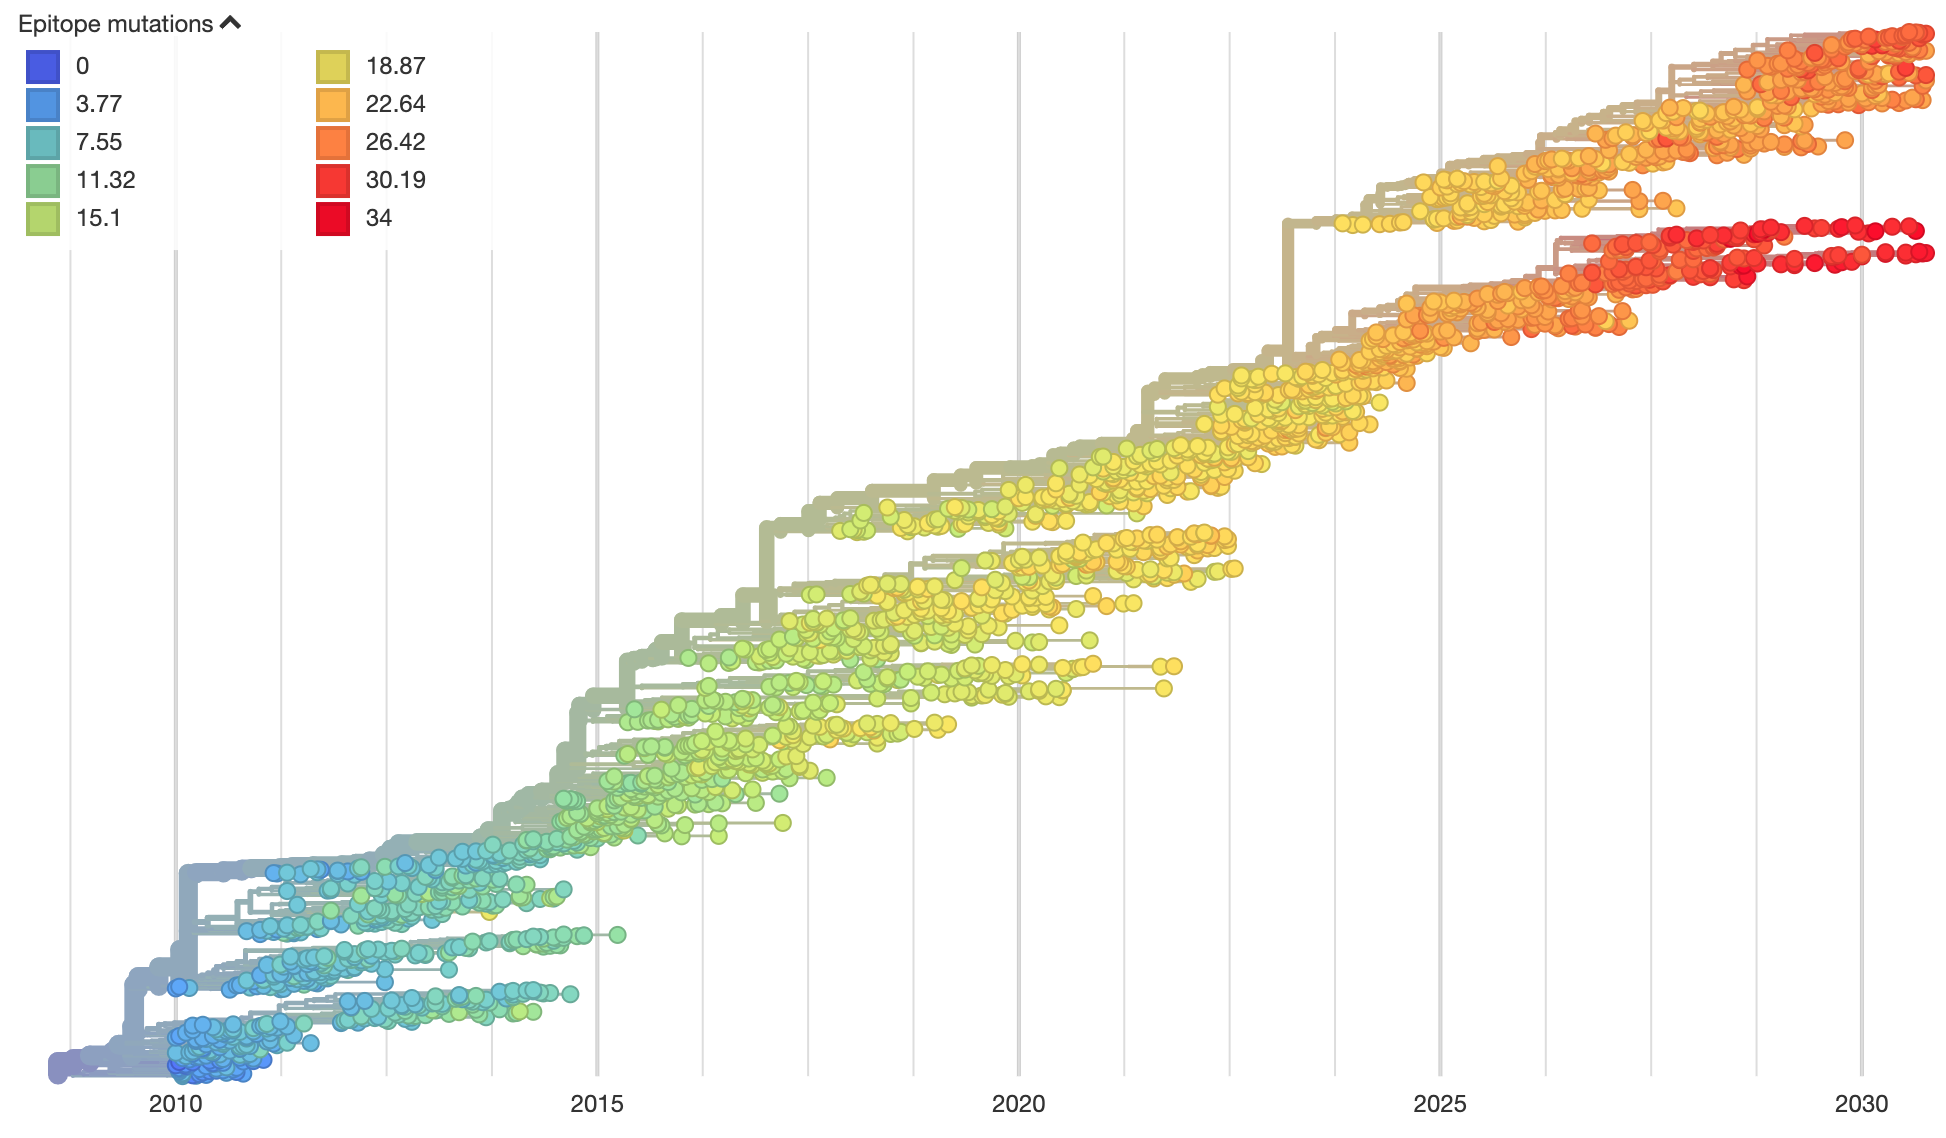
\includegraphics[width=\textwidth]{figures/simulated-h3n2-ha-phylogeny.png}
  \caption{Phylogeny of simulated A/H3N2-like HA sequences. The phylogenetic structure and rate of accumulated epitope and non-epitope mutations match patterns observed in phylogenies of natural sequences. Sample dates were annotated as the generation in the simulation divided by 100 and added to 2000, to acquire realistic date ranges that were compatible with our modeling machinery.}
  \label{sup_fig:simulated_h3n2_ha_phylogeny}
  \end{center}
\end{figure*}

\begin{figure*}[t]
  \begin{center}
  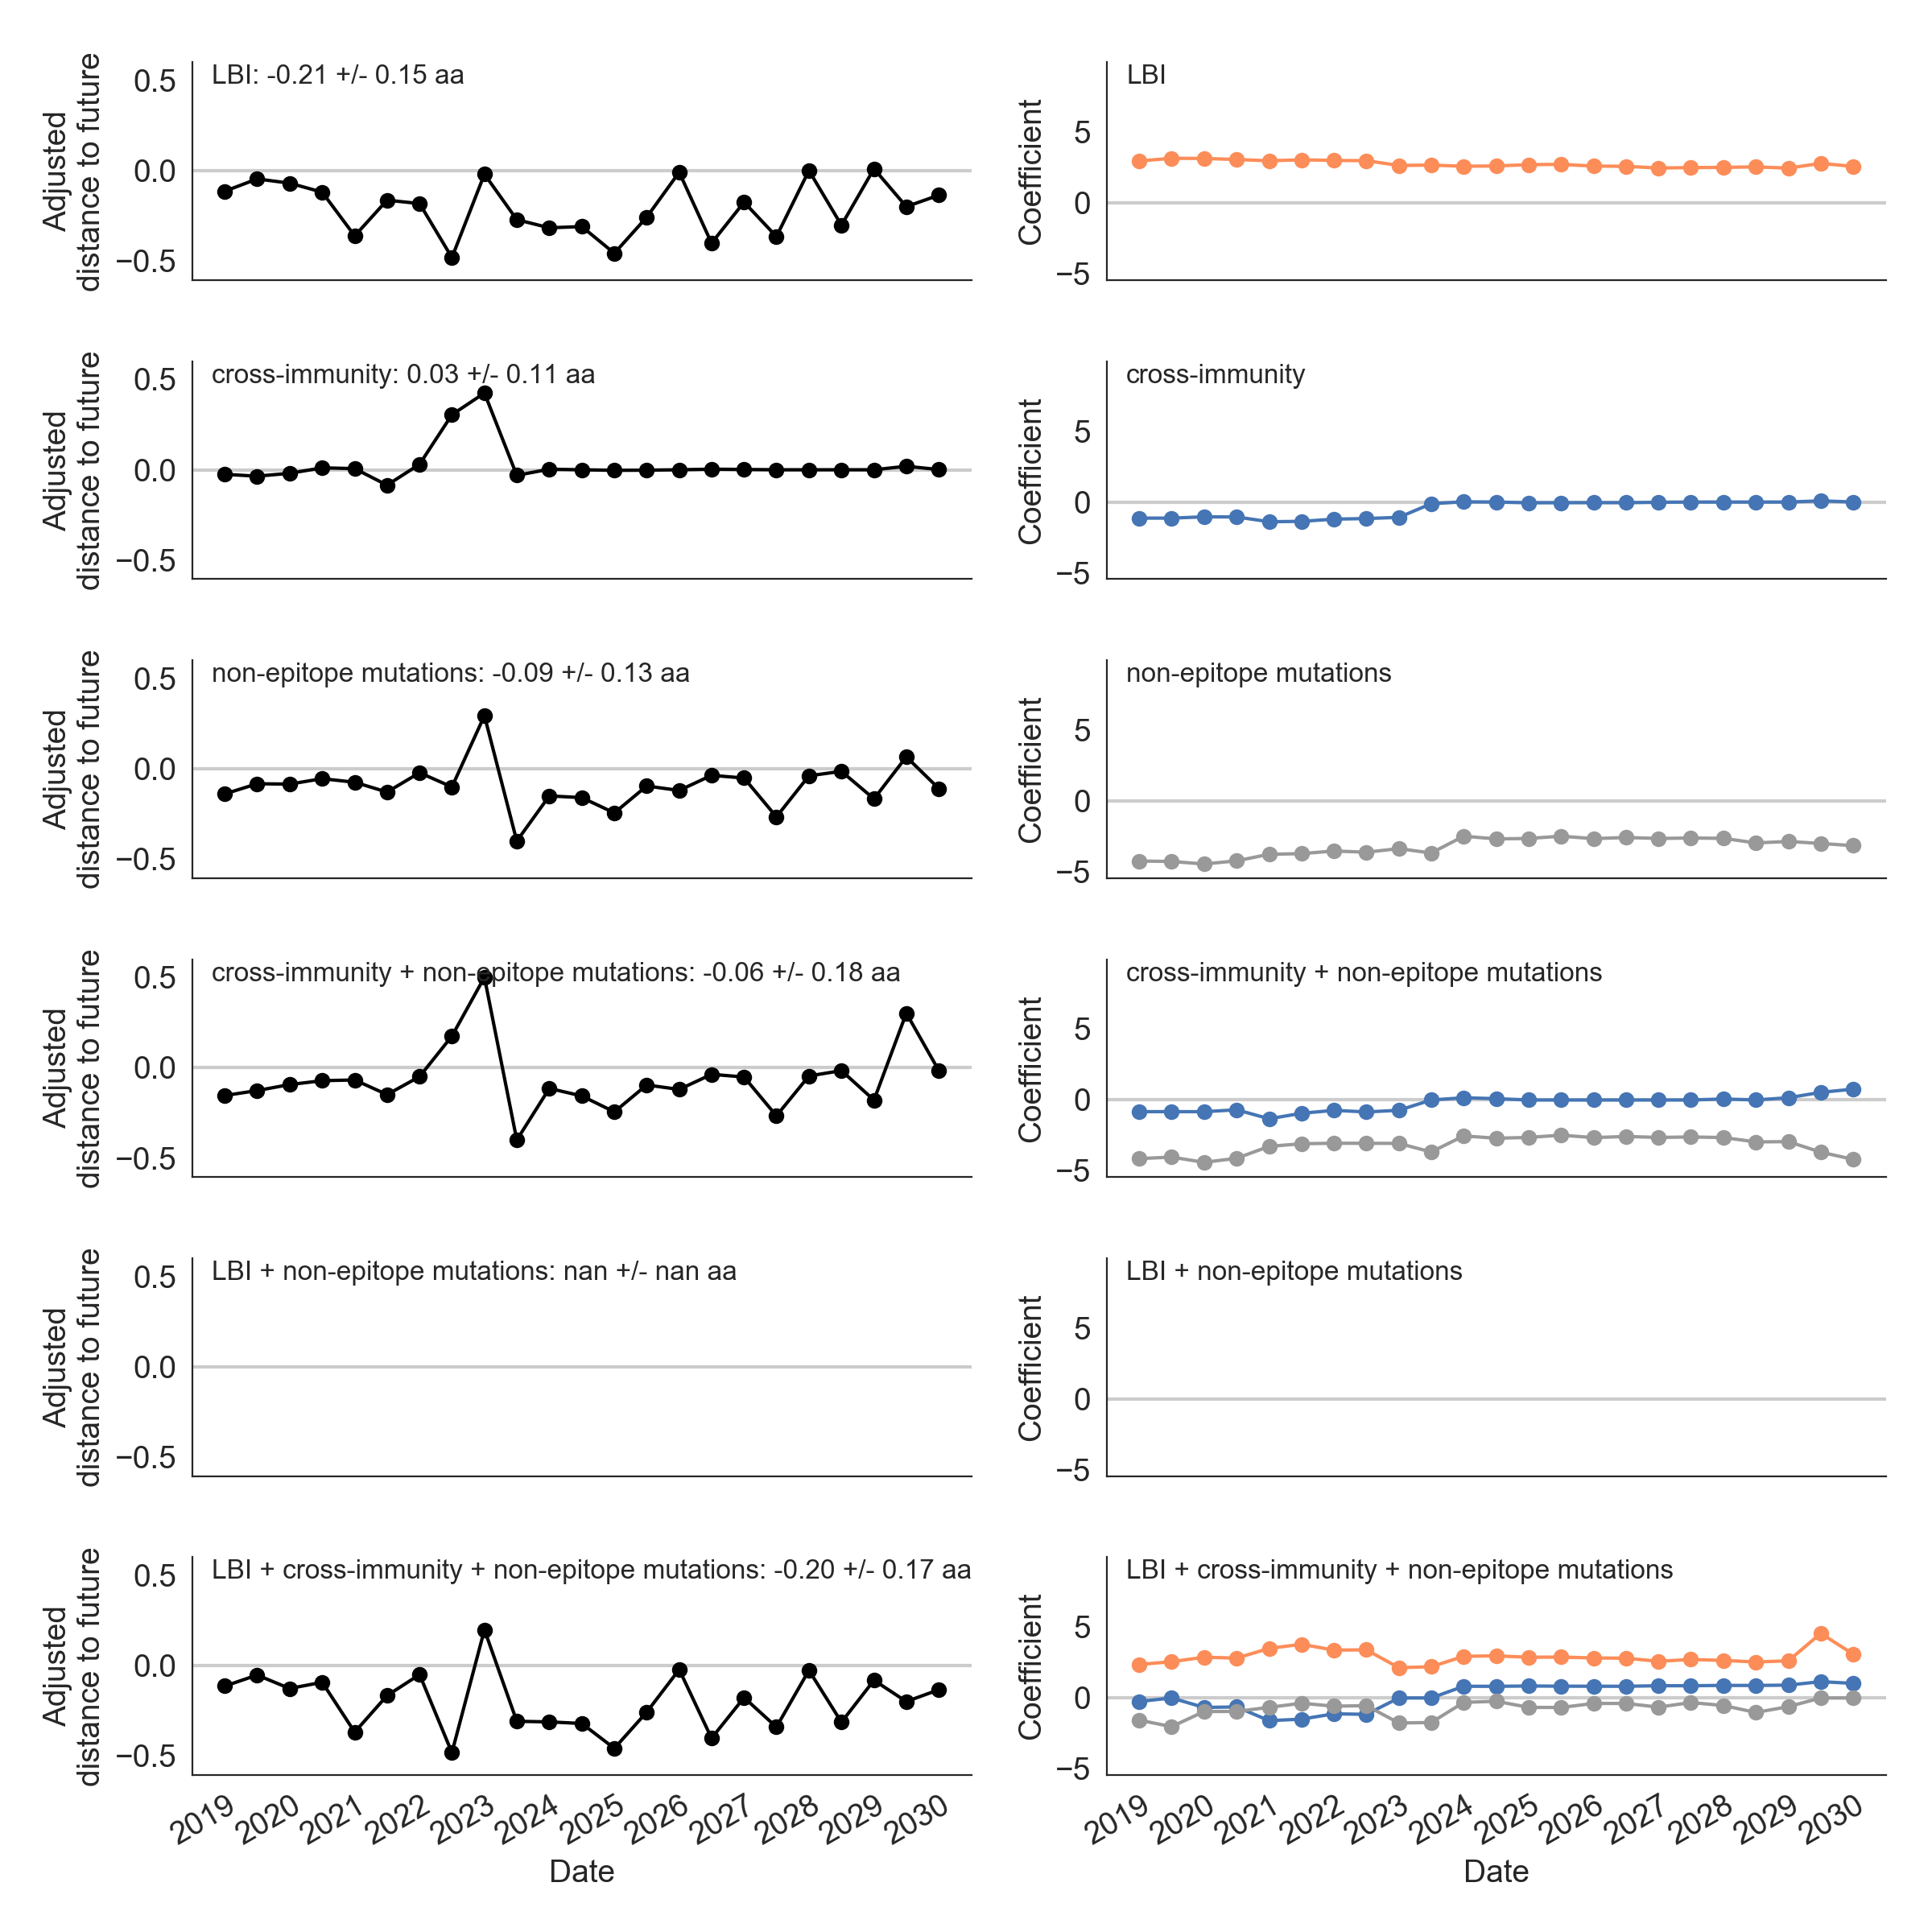
\includegraphics[width=\textwidth]{figures/composite-model-accuracy-and-coefficients-for-simulated-populations.png}
  \caption{Composite model a) accuracy and b) coefficients for simulated populations of A/H3N2-like viruses.}
  \label{sup_fig:composite_model_accuracy_and_coefficients_for_simulated_populations}
  \end{center}
\end{figure*}
